\documentclass[a4paper,12pt]{article}
\usepackage[T1]{fontenc}
\usepackage[utf8]{inputenc}
\usepackage[polish]{babel}
\usepackage{color}
\usepackage{graphicx}
\usepackage{amsmath}
\usepackage{amssymb}
\usepackage{hyperref}
\usepackage{float}
\usepackage{listings}
\usepackage[backend=biber]{biblatex}

\addbibresource{bibliografia.bib}

\lstset{
  basicstyle=\ttfamily,
  columns=flexible,
  keepspaces=true,
  showstringspaces=false,
  escapeinside={(*@}{@*)},
  literate={ą}{{\k{a}}}1
           {ć}{{\'{c}}}1
           {ę}{{\k{e}}}1
           {ł}{{\l{}}}1
           {ń}{{\'{n}}}1
           {ó}{{\'{o}}}1
           {ś}{{\'{s}}}1
           {ź}{{\'{z}}}1
           {ż}{{\.{z}}}1
           {Ą}{{\k{A}}}1
           {Ć}{{\'{C}}}1
           {Ę}{{\k{E}}}1
           {Ł}{{\L{}}}1
           {Ń}{{\'{N}}}1
           {Ó}{{\'{O}}}1
           {Ś}{{\'{S}}}1
           {Ź}{{\'{Z}}}1
           {Ż}{{\.{Z}}}1
           {"}{{\textquotedbl}}1
           {'}{{\textquotesingle}}1
           {`}{{\textasciigrave}}1
           {~}{{\textasciitilde}}1
           {^}{{\textasciicircum}}1
           {_}{{\textunderscore}}1
           {|}{{\textbar}}1
           {\{}{{\textbraceleft}}1
           {\}}{{\textbraceright}}1
           {[}{{[}}1
           {]}{{]}}1
}

\title{3. sprawozdanie z laboratorium Hurtownie Danych}
\author{Mikołaj Kubś, 272662}
\date{\today}

\begin{document}

\maketitle

\section{Zadanie 1 - funkcje grupujące}

\subsection{}

Przygotować zestawienie przedstawiające, ile pieniędzy wydali klienci na zamówienia
na przestrzeni poszczególnych lat.
Wykonaj zestawienie przy użyciu poleceń rollup, cube, grouping sets.

CUBE:

{\small
\begin{lstlisting}[
	language=SQL,
	showspaces=false,
	basicstyle=\ttfamily,
	numbers=left,
	numberstyle=\tiny,
	commentstyle=\color{green},
	tabsize=2
]
SELECT
    CASE 
        WHEN GROUPING(Person.BusinessEntityID) = 1 THEN '1. total sum'
        ELSE CONCAT(MIN(Person.FirstName), ' ', MIN(Person.LastName))
    END AS FullName,
    YEAR(OrderDate) AS OrderYear,
    SUM(TotalDue) AS TotalSales
FROM Sales.SalesOrderHeader
JOIN Sales.Customer ON Customer.CustomerID = SalesOrderHeader.CustomerID
JOIN Person.Person ON Person.BusinessEntityID = Customer.PersonID
GROUP BY 
    CUBE(Person.BusinessEntityID, YEAR(OrderDate))
ORDER BY 
    FullName, OrderYear
\end{lstlisting}}

\begin{figure}[H]
  \centering
  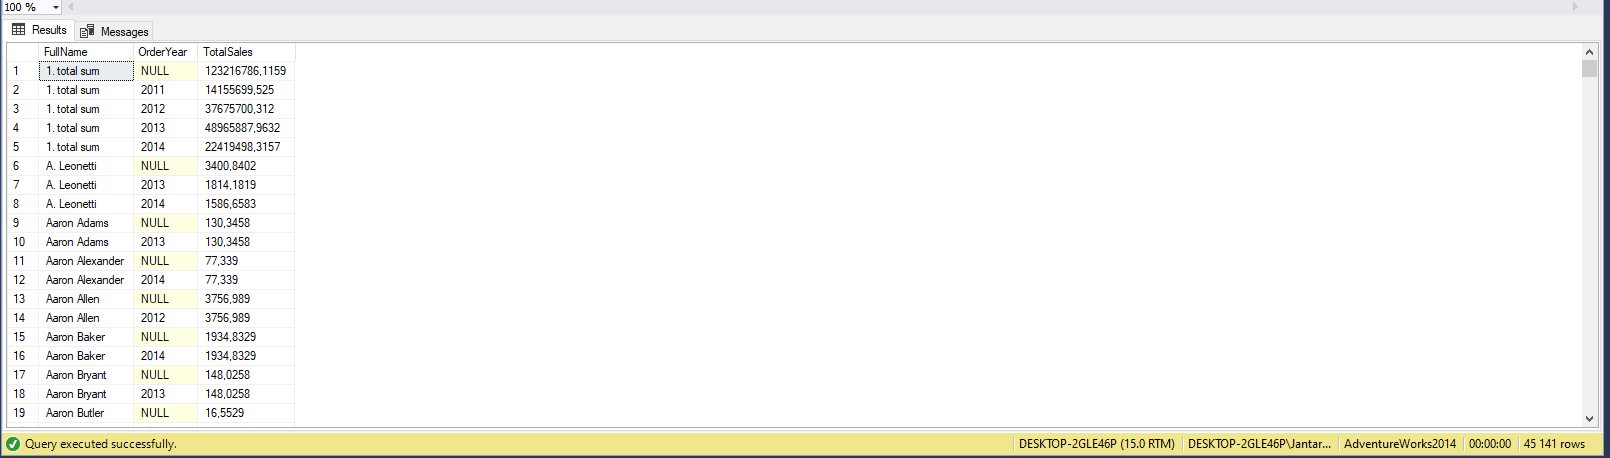
\includegraphics[width=1.0\textwidth]{images/1.1_cube.png}
  \caption{Wynik kwerendy 1.1: CUBE}
\end{figure}

ROLLUP:

{\small
\begin{lstlisting}[
	language=SQL,
	showspaces=false,
	basicstyle=\ttfamily,
	numbers=left,
	numberstyle=\tiny,
	commentstyle=\color{green},
	tabsize=2
]
SELECT
    CASE 
        WHEN GROUPING(YEAR(OrderDate)) = 1 AND 
        GROUPING(Person.BusinessEntityID) = 1 
        THEN '1. total sum'
        WHEN GROUPING(YEAR(OrderDate)) = 1 THEN 
        CONCAT(MIN(Person.FirstName), ' ', MIN(Person.LastName), ' (total)')
        ELSE MIN(CONCAT(Person.FirstName, ' ', Person.LastName))
    END AS FullName,
    YEAR(OrderDate) AS OrderYear,
    SUM(TotalDue) AS TotalSales
FROM Sales.SalesOrderHeader
JOIN Sales.Customer ON Customer.CustomerID = SalesOrderHeader.CustomerID
JOIN Person.Person ON Person.BusinessEntityID = Customer.PersonID
GROUP BY 
    ROLLUP(Person.BusinessEntityID, YEAR(OrderDate))
ORDER BY 
    FullName, OrderYear
\end{lstlisting}}

\begin{figure}[H]
  \centering
  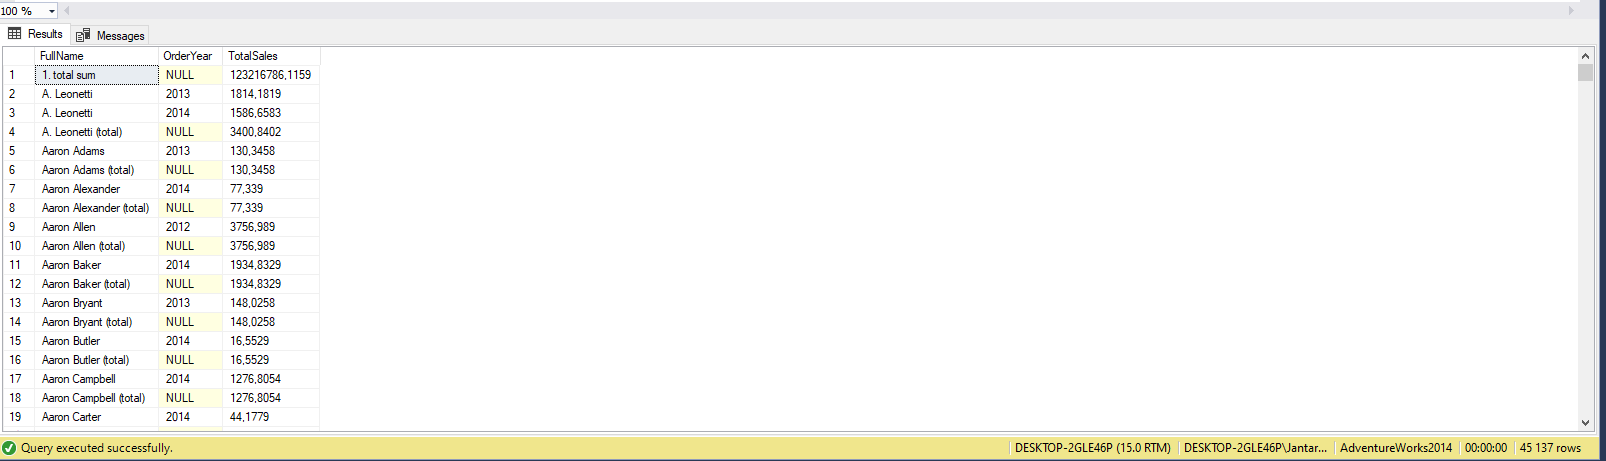
\includegraphics[width=1.0\textwidth]{images/1.1_rollup.png}
  \caption{Wynik kwerendy 1.1: ROLLUP}
\end{figure}

GROUPING SETS:

{\small
\begin{lstlisting}[
	language=SQL,
	showspaces=false,
	basicstyle=\ttfamily,
	numbers=left,
	numberstyle=\tiny,
	commentstyle=\color{green},
	tabsize=2
]
SELECT
    MIN(CONCAT(Person.FirstName, ' ', Person.LastName)) AS FullName,	
    YEAR(OrderDate) AS OrderYear,
    SUM(TotalDue) AS TotalDue
FROM Sales.SalesOrderHeader
JOIN Sales.Customer ON Customer.CustomerID = SalesOrderHeader.CustomerID
JOIN Person.Person ON Person.BusinessEntityID = Customer.PersonID
GROUP BY GROUPING SETS
    (
		(Person.BusinessEntityID),
        (YEAR(OrderDate), Person.BusinessEntityID)
    )
ORDER BY FullName, OrderYear
\end{lstlisting}}

\begin{figure}[H]
  \centering
  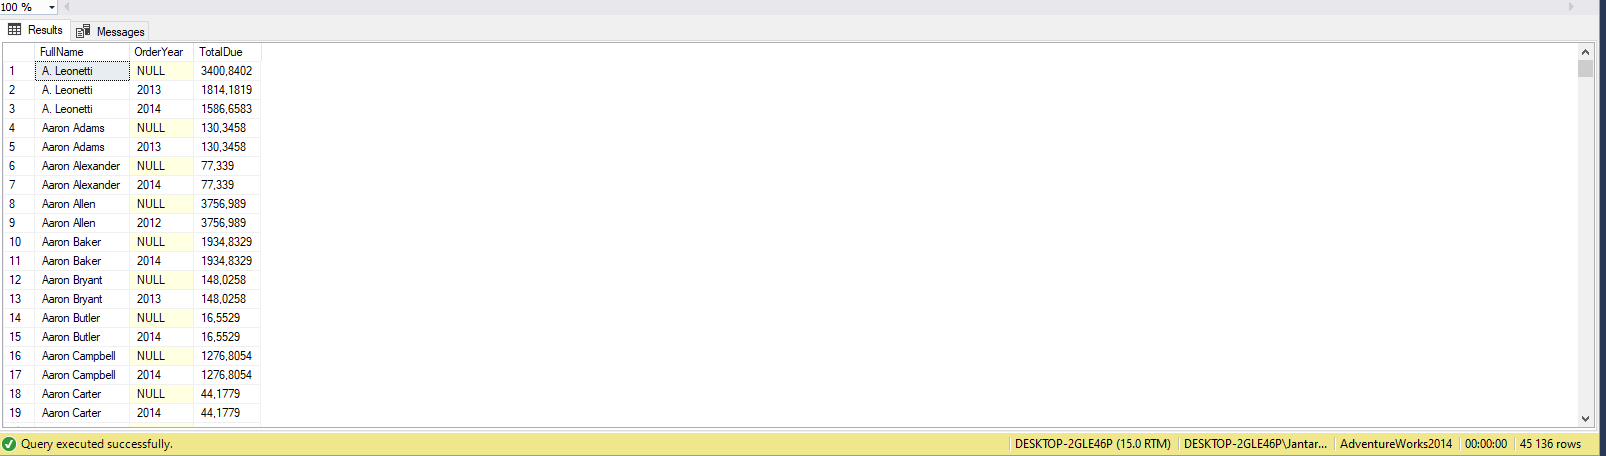
\includegraphics[width=1.0\textwidth]{images/1.1_grouping.png}
  \caption{Wynik kwerendy 1.1: GROUPING SETS}
\end{figure}

\subsection{}

Przygotować zestawienie przedstawiające łączną kwotę zniżek z podziałem na katego-
rie, produkty oraz lata.

  {\small
    \begin{lstlisting}[
	language=SQL,
	showspaces=false,
	basicstyle=\ttfamily,
	numbers=left,
	numberstyle=\tiny,
	commentstyle=\color{green},
	tabsize=2
]
SELECT 
    ProductCategory.Name AS Kategoria, 
    ISNULL(Product.Name, '1. total') AS "Nazwa produktu", 
    ISNULL(CAST(YEAR(OrderDate) AS VARCHAR), 'total') AS Rok, 
    SUM(UnitPrice * OrderQty - LineTotal) AS "Suma rabatu" 
FROM Sales.SalesOrderDetail
JOIN Sales.SalesOrderHeader ON SalesOrderHeader.SalesOrderID = 
    SalesOrderDetail.SalesOrderID
JOIN Production.Product ON SalesOrderDetail.ProductID = Product.ProductID
LEFT JOIN Production.ProductSubcategory ON 
    Product.ProductSubcategoryID = ProductSubcategory.ProductSubcategoryID
LEFT JOIN Production.ProductCategory ON 
    ProductSubcategory.ProductCategoryID = ProductCategory.ProductCategoryID
GROUP BY 
    CUBE(Product.Name, YEAR(OrderDate)),
	ProductCategory.Name
ORDER BY 
    Kategoria, "Nazwa produktu", Rok
\end{lstlisting}}

\begin{figure}[H]
  \centering
  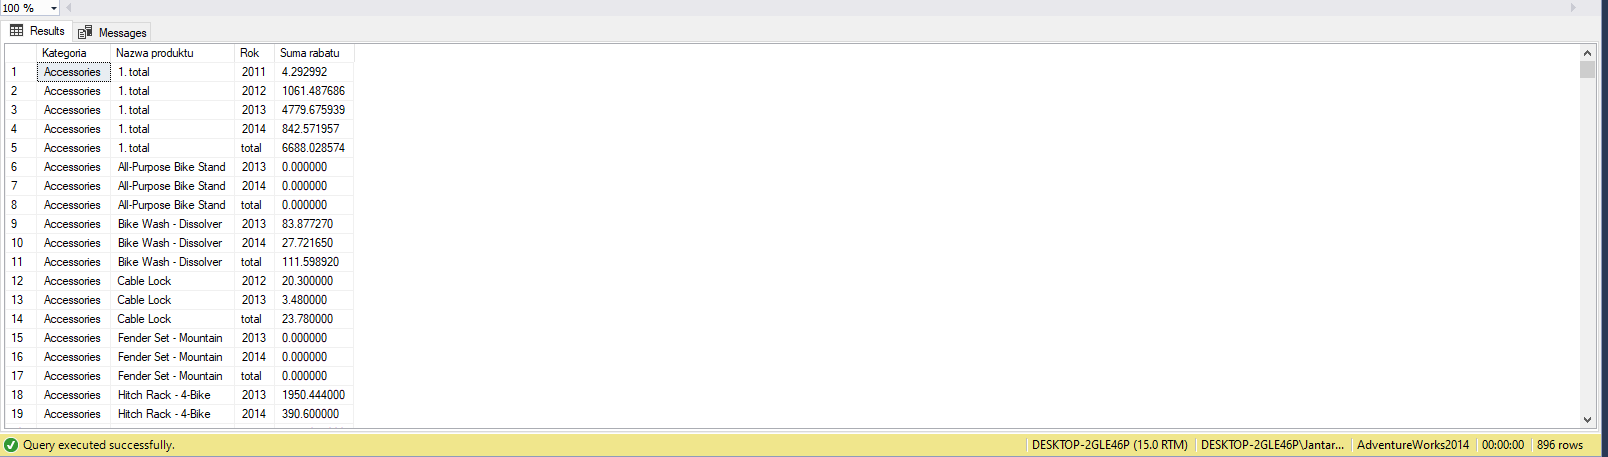
\includegraphics[width=1.0\textwidth]{images/1.2.png}
  \caption{Wynik kwerendy 1.2}
\end{figure}

\section{Zadanie 2 - funkcje okienkowe}

\subsection{}

Dla kategorii ‘Bikes’ przygotuj zestawienie prezentujące procentowy udział kwot
sprzedaży produktów tej kategorii w poszczególnych latach w stosunku do łącznej
kwoty sprzedaży dla tej kategorii. W zadaniu wykorzystaj funkcje okna.
Wykonaj podobne zestawienia dla pozostałych kategorii.

  {\small
    \begin{lstlisting}[
	language=SQL,
	showspaces=false,
	basicstyle=\ttfamily,
	numbers=left,
	numberstyle=\tiny,
	commentstyle=\color{green},
	tabsize=2
]
SELECT 
    ISNULL(ProductCategory.Name, 'Total') AS "Nazwa kategorii",
    YEAR(SalesOrderHeader.OrderDate) AS Rok,
	  SUM(SalesOrderDetail.LineTotal) AS "Suma sprzedazy",
    CAST(ROUND(SUM(SalesOrderDetail.LineTotal) / SUM(SUM(SalesOrderDetail.LineTotal)) 
    OVER (PARTITION BY ProductCategory.Name) * 100, 2) AS DECIMAL(10,2)) 
    AS "Procent sprzedazy dla kategorii"
FROM 
    Sales.SalesOrderDetail
    JOIN Sales.SalesOrderHeader ON 
      SalesOrderDetail.SalesOrderID = SalesOrderHeader.SalesOrderID
    JOIN Production.Product ON 
      SalesOrderDetail.ProductID = Product.ProductID
    JOIN Production.ProductSubcategory ON 
      Product.ProductSubcategoryID = ProductSubcategory.ProductSubcategoryID
    JOIN Production.ProductCategory ON 
      ProductSubcategory.ProductCategoryID = ProductCategory.ProductCategoryID
GROUP BY 
    YEAR(SalesOrderHeader.OrderDate),
    CUBE(ProductCategory.Name)
ORDER BY 
    COALESCE(ProductCategory.Name, 'Total') DESC,
    YEAR(SalesOrderHeader.OrderDate);
\end{lstlisting}}

\begin{figure}[H]
  \centering
  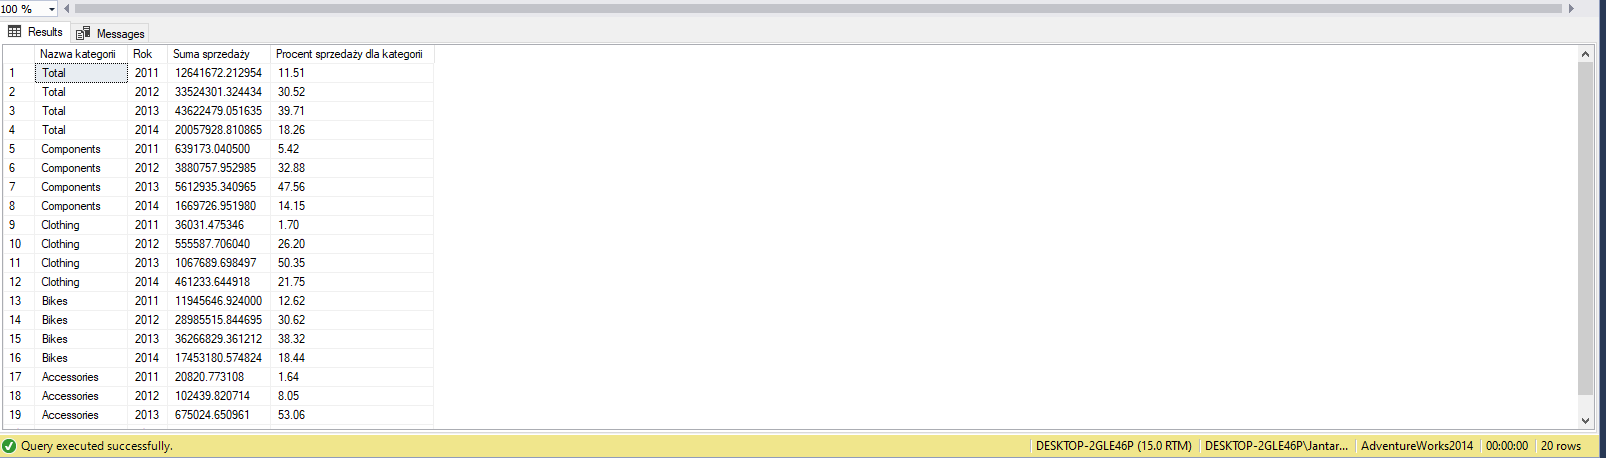
\includegraphics[width=1.0\textwidth]{images/2.1.png}
  \caption{Wynik kwerendy 2.1}
\end{figure}

\subsection{}

Przygotuj zestawienie dla sprzedawców z podziałem na lata i miesiące prezentujące
liczbę obsłużonych przez nich zamówień w ciągu roku, w ciągu roku narastająco oraz
sumarycznie w obecnym i poprzednim miesiącu. W zadaniu wykorzystaj funkcje okna.

  {\small
    \begin{lstlisting}[
	language=SQL,
	showspaces=false,
	basicstyle=\ttfamily,
	numbers=left,
	numberstyle=\tiny,
	commentstyle=\color{green},
	tabsize=2
]
SELECT 
    Person.FirstName + ' ' + Person.LastName AS [Imie i nazwisko],
    YEAR(SalesOrderHeader.OrderDate) AS [Rok],
    MONTH(SalesOrderHeader.OrderDate) AS [Miesiac],
    COUNT(*) AS [W miesiacu],
    SUM(COUNT(*)) OVER 
      (PARTITION BY
        Person.BusinessEntityID, 
        YEAR(SalesOrderHeader.OrderDate)) 
    AS [W roku],
    SUM(COUNT(*)) OVER 
      (PARTITION BY 
        Person.BusinessEntityID, 
        YEAR(SalesOrderHeader.OrderDate)                 
      ORDER BY MONTH(SalesOrderHeader.OrderDate)) 
    AS [W roku narastajaco],
    COUNT(*) + LAG(COUNT(*), 1, 0) OVER 
      (PARTITION BY Person.BusinessEntityID 
      ORDER BY YEAR(SalesOrderHeader.OrderDate), MONTH(SalesOrderHeader.OrderDate)) 
    AS [Obecny i poprzedni miesiac]
FROM 
    Sales.SalesOrderHeader
    JOIN Sales.SalesPerson ON 
      SalesOrderHeader.SalesPersonID = SalesPerson.BusinessEntityID
    JOIN Person.Person ON 
      SalesPerson.BusinessEntityID = Person.BusinessEntityID
GROUP BY 
    Person.BusinessEntityID,
    Person.FirstName,
    Person.LastName,
    YEAR(SalesOrderHeader.OrderDate),
    MONTH(SalesOrderHeader.OrderDate)
ORDER BY 
    [Imie i nazwisko],
    [Rok],
    [Miesiac];
\end{lstlisting}}

\begin{figure}[H]
  \centering
  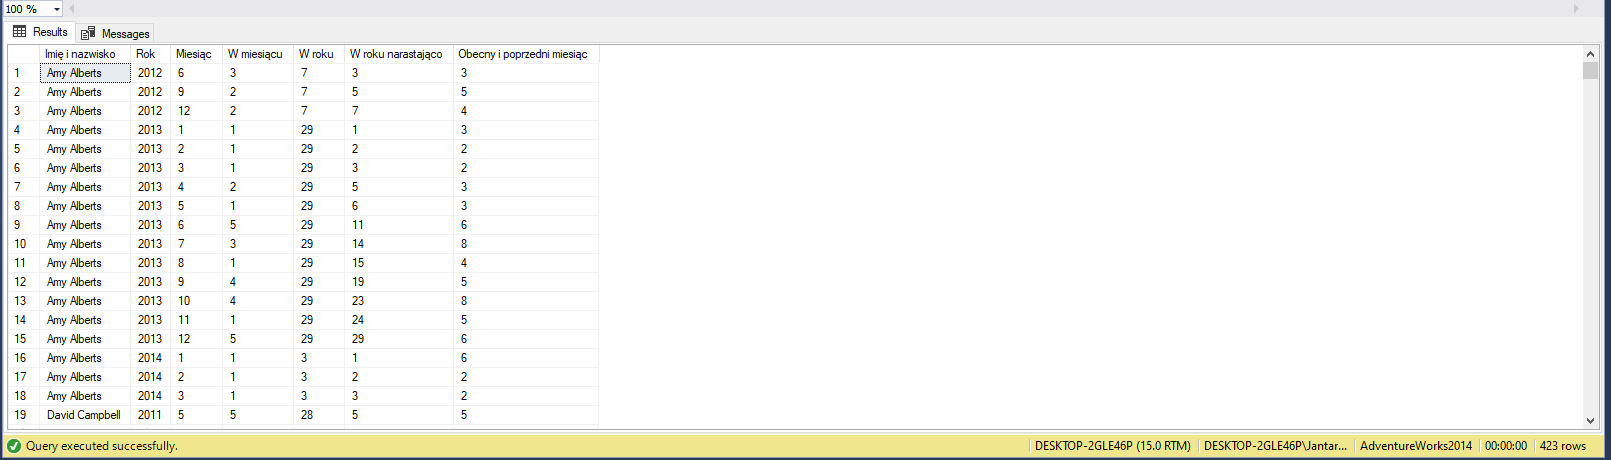
\includegraphics[width=1.0\textwidth]{images/2.2.png}
  \caption{Wynik kwerendy 2.2}
\end{figure}

\subsection{}

Przygotuj ranking klientów w zależności od liczby zakupionych produktów. Porównaj rozwiązania uzyskane przez funkcje rank i dense\_rank.

RANK:

{\small
\begin{lstlisting}[
	language=SQL,
	showspaces=false,
	basicstyle=\ttfamily,
	numbers=left,
	numberstyle=\tiny,
	commentstyle=\color{green},
	tabsize=2
]
SELECT 
	Customer.CustomerID AS "ID",
	Person.FirstName AS "Imie",
	Person.LastName AS "Nazwisko",
	COUNT(*) AS "Liczba transakcji",
	RANK() OVER(ORDER BY COUNT(*) DESC) AS "Ranking"
FROM Sales.Customer
RIGHT JOIN Sales.SalesOrderHeader ON 
  SalesOrderHeader.CustomerID = Customer.CustomerID
RIGHT JOIN Sales.SalesOrderDetail ON 
  SalesOrderDetail.SalesOrderID = SalesOrderHeader.SalesOrderID
JOIN Person.Person ON Person.BusinessEntityID = Customer.PersonID
GROUP BY Customer.CustomerID, Person.FirstName, Person.LastName
ORDER BY COUNT(*) DESC
\end{lstlisting}}

\begin{figure}[H]
  \centering
  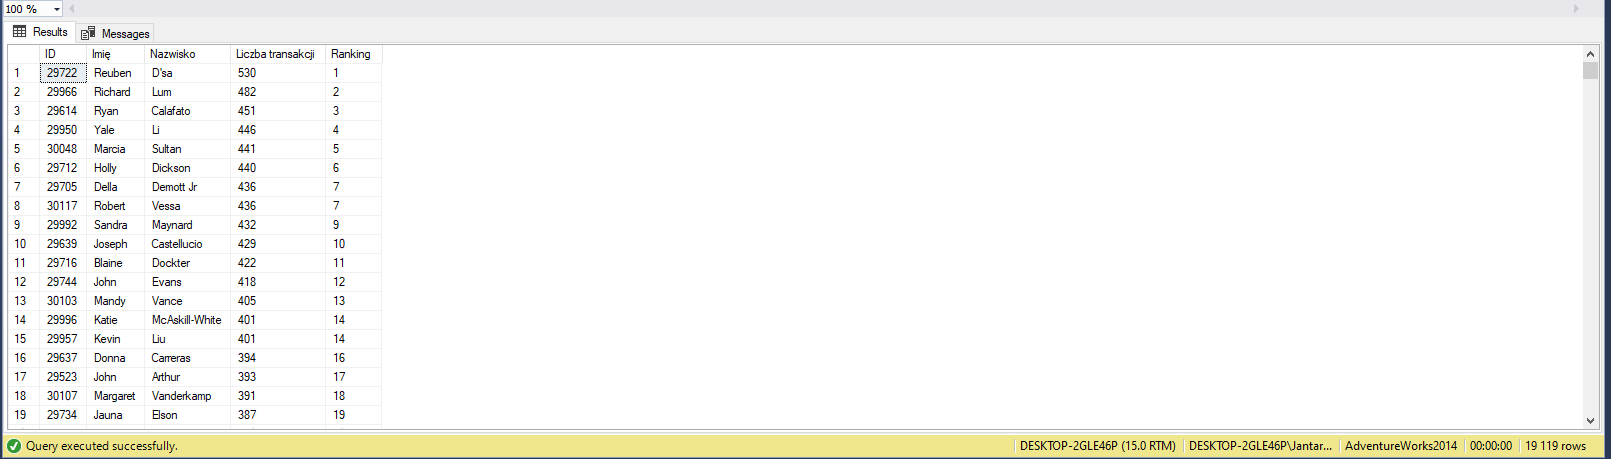
\includegraphics[width=1.0\textwidth]{images/2.3.png}
  \caption{Wynik kwerendy 2.3: RANK}
\end{figure}

DENSE\_RANK:

{\small
  \begin{lstlisting}[
	language=SQL,
	showspaces=false,
	basicstyle=\ttfamily,
	numbers=left,
	numberstyle=\tiny,
	commentstyle=\color{green},
	tabsize=2
]
SELECT 
	Customer.CustomerID AS "ID",
	Person.FirstName AS "Imie",
	Person.LastName AS "Nazwisko",
	COUNT(*) AS "Liczba transakcji",
	DENSE_RANK() OVER(ORDER BY COUNT(*) DESC) AS "Ranking"
FROM Sales.Customer
RIGHT JOIN Sales.SalesOrderHeader ON 
  SalesOrderHeader.CustomerID = Customer.CustomerID
RIGHT JOIN Sales.SalesOrderDetail ON 
  SalesOrderDetail.SalesOrderID = SalesOrderHeader.SalesOrderID
JOIN Person.Person ON Person.BusinessEntityID = Customer.PersonID
GROUP BY Customer.CustomerID, Person.FirstName, Person.LastName
ORDER BY COUNT(*) DESC
\end{lstlisting}}

\begin{figure}[H]
  \centering
  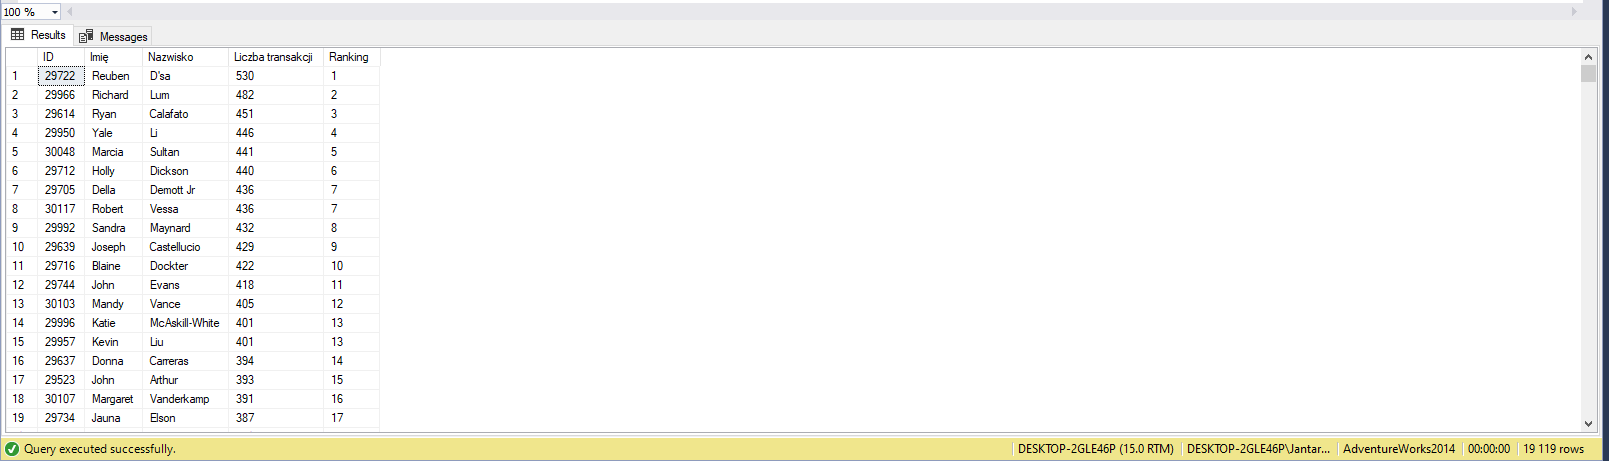
\includegraphics[width=1.0\textwidth]{images/2.3_dense.png}
  \caption{Wynik kwerendy 2.3: DENSE\_RANK}
\end{figure}

\subsection{}

Przygotuj ranking produktów w zależności od średniej liczby sprzedanych sztuk. Wyróżnij 3 (prawie równoliczne) grupy produktów: sprzedających się najlepiej, średnio i najsłabiej.

{\small
\begin{lstlisting}[
	language=SQL,
	showspaces=false,
	basicstyle=\ttfamily,
	numbers=left,
	numberstyle=\tiny,
	commentstyle=\color{green},
	tabsize=2
]
WITH ProductsRanked AS 
(
	SELECT 
		Product.ProductID AS "ID produktu",
		Product.Name AS "Nazwa produktu",
		SUM(SalesOrderDetail.OrderQty) AS "Suma liczby sprzedanych sztuk",
		AVG(CAST(SalesOrderDetail.OrderQty AS DECIMAL(10,2))) 
    AS "Srednia liczba sprzedanych sztuk",
		NTILE(3) OVER (ORDER BY AVG(CAST(SalesOrderDetail.OrderQty AS FLOAT)) DESC) 
    AS "Numer grupy"
	FROM Production.Product
	JOIN Sales.SalesOrderDetail 
    ON SalesOrderDetail.ProductID = Product.ProductID
	GROUP BY Product.ProductID, Product.Name
)
SELECT 
	ProductsRanked.[ID produktu],
	ProductsRanked.[Nazwa produktu],
	ProductsRanked.[Suma liczby sprzedanych sztuk],
	ProductsRanked.[Srednia liczba sprzedanych sztuk],
	CASE 
    WHEN "Numer grupy" = 1 THEN 'Najlepiej sprzedajace sie'
    WHEN "Numer grupy" = 2 THEN 'Srednio sprzedajace sie'
    WHEN "Numer grupy" = 3 THEN 'Najslabiej sprzedajace sie'
  END AS SalesCategory
FROM ProductsRanked
ORDER BY ProductsRanked.[Srednia liczba sprzedanych sztuk] DESC
\end{lstlisting}}

\begin{figure}[H]
  \centering
  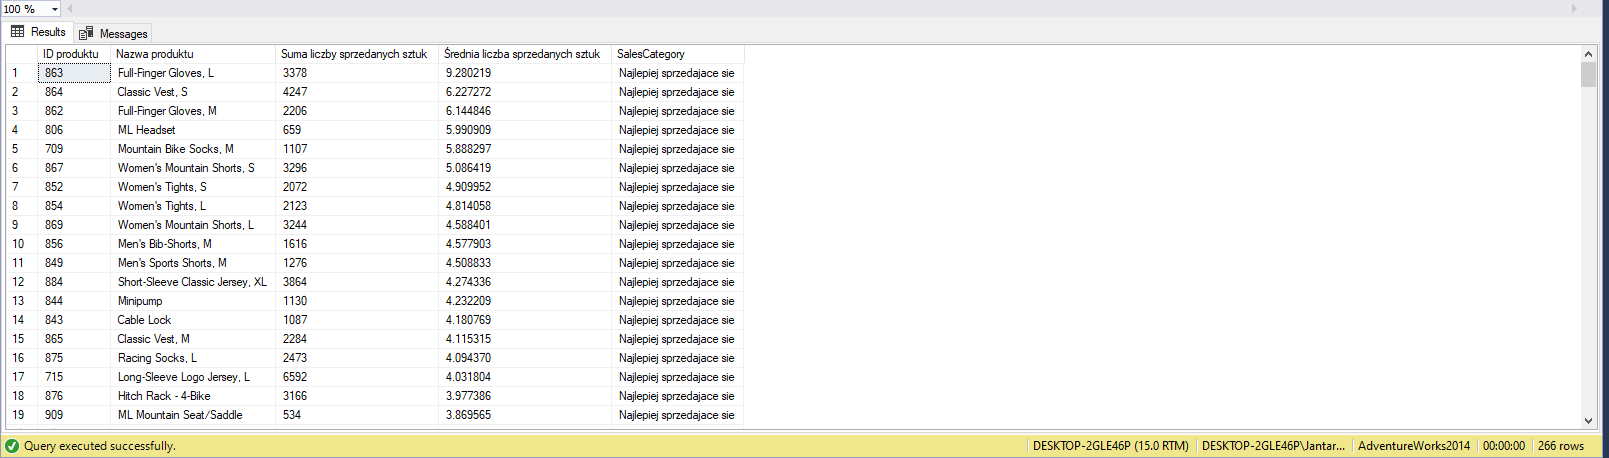
\includegraphics[width=1.0\textwidth]{images/2.4.png}
  \caption{Wynik kwerendy 2.4}
\end{figure}

\begin{figure}[H]
  \centering
  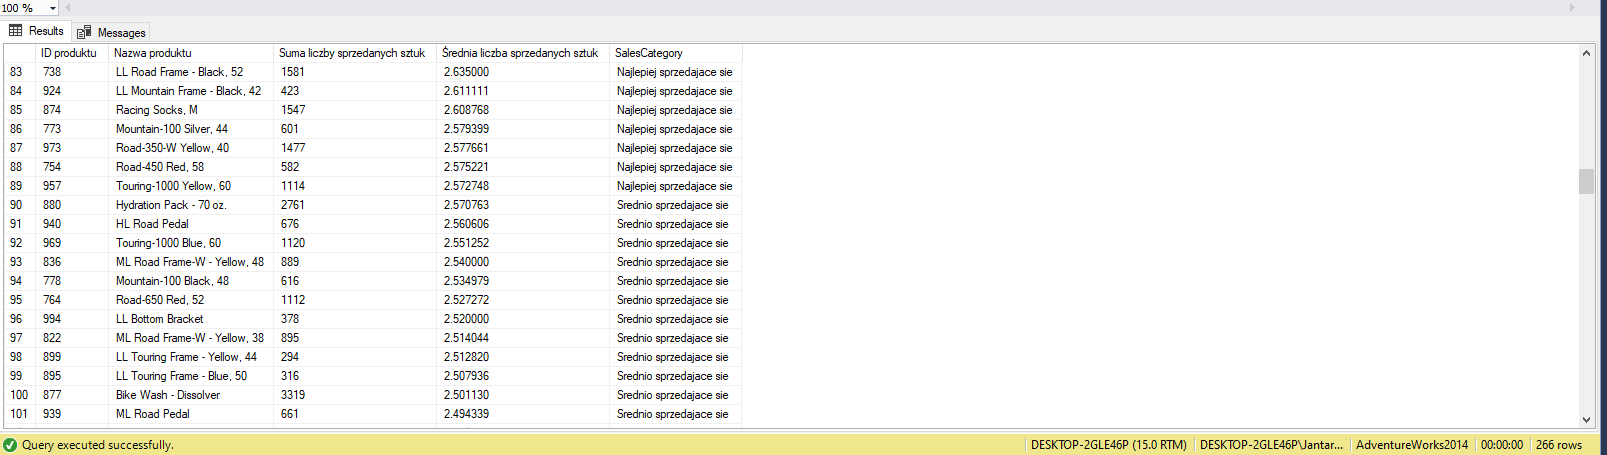
\includegraphics[width=1.0\textwidth]{images/2.4_avg_selling.png}
  \caption{Widok przejścia do części średnio sprzedającej się}
\end{figure}

\section{Zadanie 3 - profilowanie danych}

Po próbach analizy w SSIS uzyskano tylko część rezultatów.

\begin{figure}[H]
  \centering
  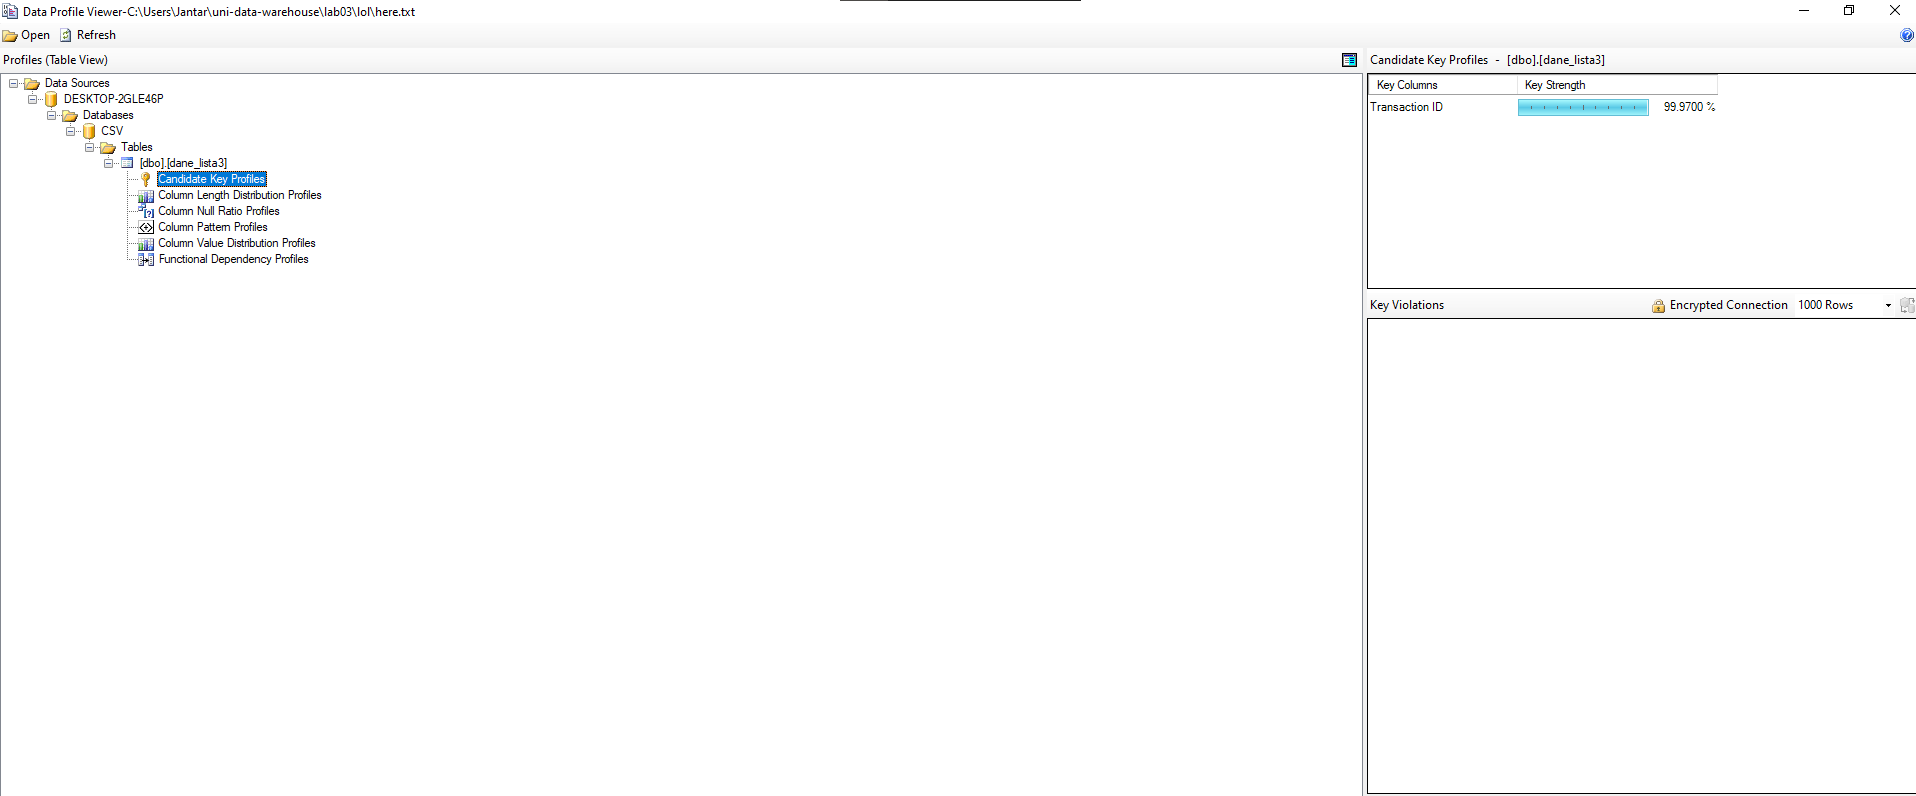
\includegraphics[width=1.0\textwidth]{images/ssis_1.png}
  \caption{Profil kolumny kandydującej}
\end{figure}

\begin{figure}[H]
  \centering
  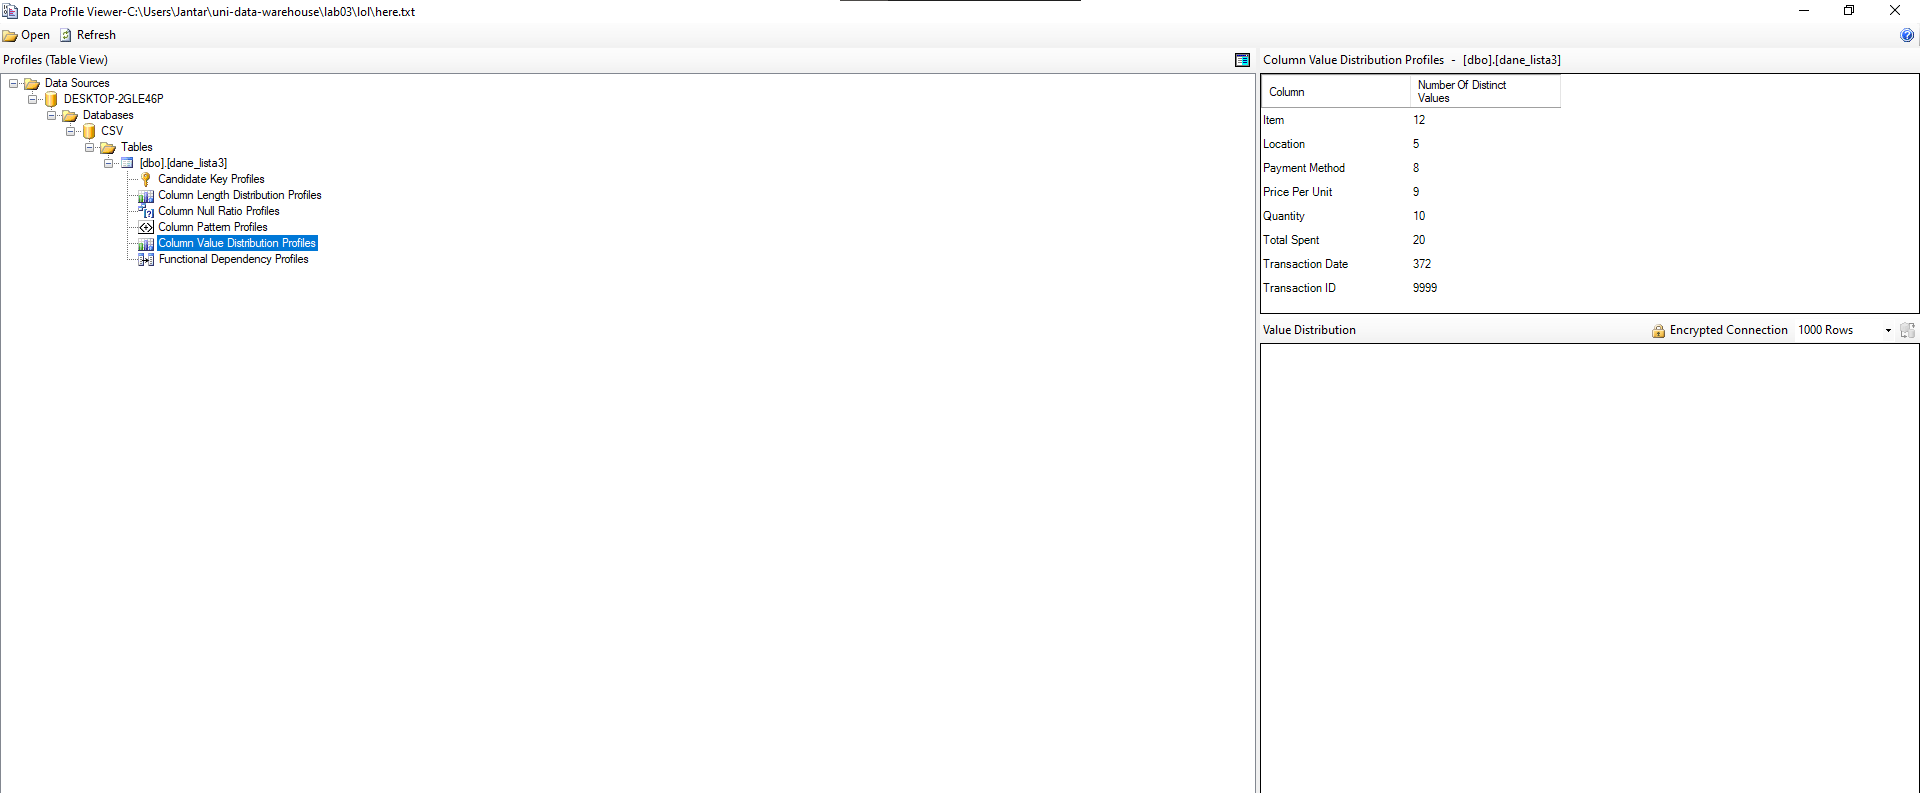
\includegraphics[width=1.0\textwidth]{images/ssis_2.png}
  \caption{Liczba unikatowych wartości w kolumnach}
\end{figure}

Z powodu problemów technicznych resztę analizy przeprowadzono używając \textit{Pythona} oraz bibliotek \textit{Pandas} i \textit{ydata\_profiling}.

\begin{lstlisting}[language=Python, basicstyle=\ttfamily\small, numbers=left, numberstyle=\tiny, commentstyle=\color{green}]
import pandas as pd
from ydata_profiling import ProfileReport
from os import path

pd.set_option('display.max_columns', None)
pd.set_option('display.width', None)
pd.set_option('display.colheader_justify', 'left')

dir_path: str = path.dirname(path.realpath(__file__))

df: pd.DataFrame = pd.read_csv(path.join(dir_path, "dane_lista3.csv"))

profile = ProfileReport(df, explorative=True)

profile.to_file(path.join(dir_path, "python_results.html"))

df['Transaction ID'] = df['Transaction ID'].astype('str')
df['Item'] = df['Item'].astype('str')
df['Quantity'] = pd.to_numeric(df['Quantity'], errors='coerce')
df['Price Per Unit'] = pd.to_numeric(df['Price Per Unit'], errors='coerce')
df['Total Spent'] = pd.to_numeric(df['Total Spent'], errors='coerce')
df['Payment Method'] = df['Payment Method'].astype('str')
df['Location'] = df['Location'].astype('str')
df['Transaction Date'] = pd.to_datetime(
    df['Transaction Date'], errors='coerce')

profile = ProfileReport(df, explorative=True)

profile.to_file(path.join(dir_path, "python_results_good_data_types.html"))

df["Wrong Total"] = (
    df["Quantity"].notnull() &
    df["Price Per Unit"].notnull() &
    df["Total Spent"].notnull() &
    (df["Quantity"] * df["Price Per Unit"] != df["Total Spent"])
)
print(f"Liczba źle policzonych Total Spent: {df['Wrong Total'].sum()}")
print(df[df["Wrong Total"]])  
\end{lstlisting}

\subsection{Transaction ID}

\begin{figure}[H]
  \centering
  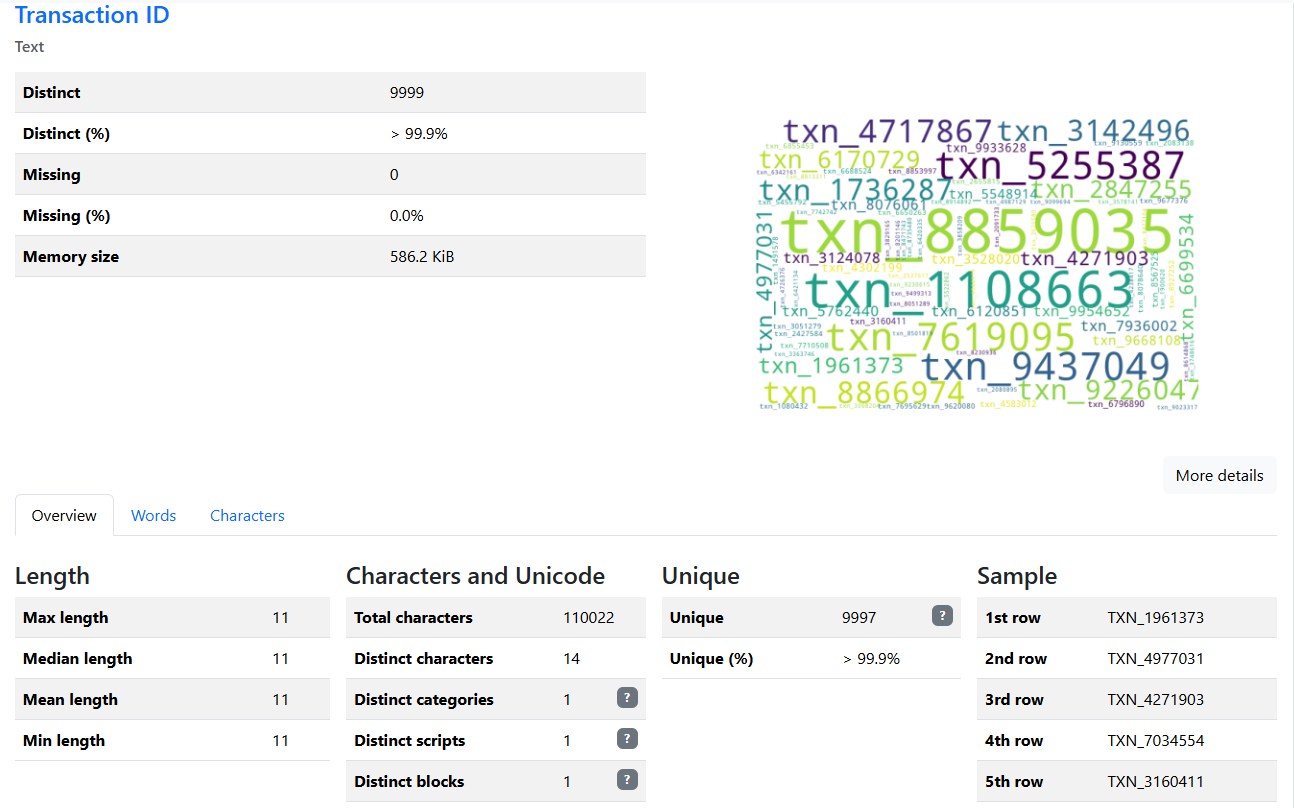
\includegraphics[width=0.65\textwidth]{images/py_1.png}
  \caption{Profil kolumny \textit{Transaction ID}}
\end{figure}

Tak jak też wywnioskowano wcześniej, jest to jedyna kolumna nadająca się na klucz kandydujący. Są w niej tylko 3 duplikaty. Zawsze ma też tą samą długość - 11 znaków.

\subsection{Item}

\begin{figure}[H]
  \centering
  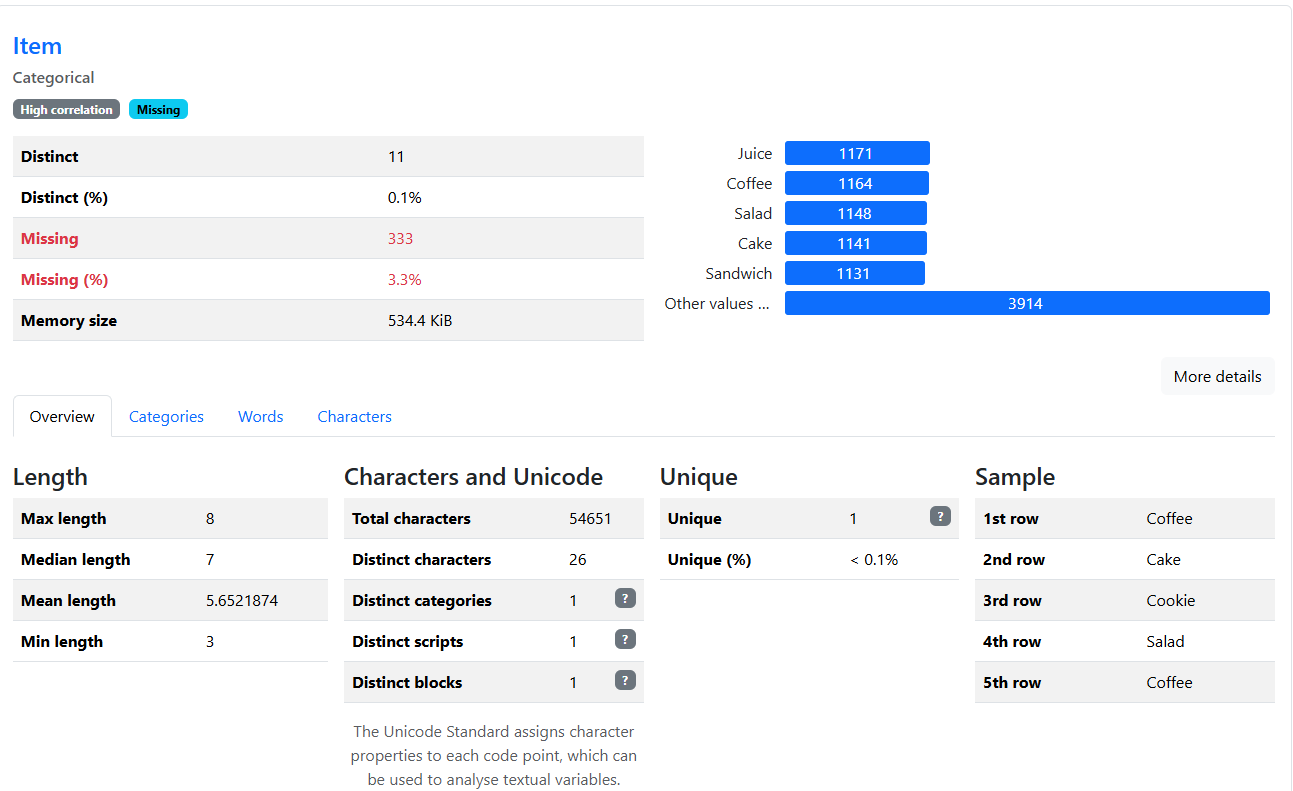
\includegraphics[width=0.65\textwidth]{images/py_2.png}
  \caption{Profil kolumny \textit{Item}}
\end{figure}

Kolumna jest kategoryczna i przypisuje transakcjom kategorię kupionego towaru. W 3.3\% wierszy brakuje wartości. Dodatkowo w 3.4\% to \textit{UNKNOWN}.

\subsection{Quantity}

\begin{figure}[H]
  \centering
  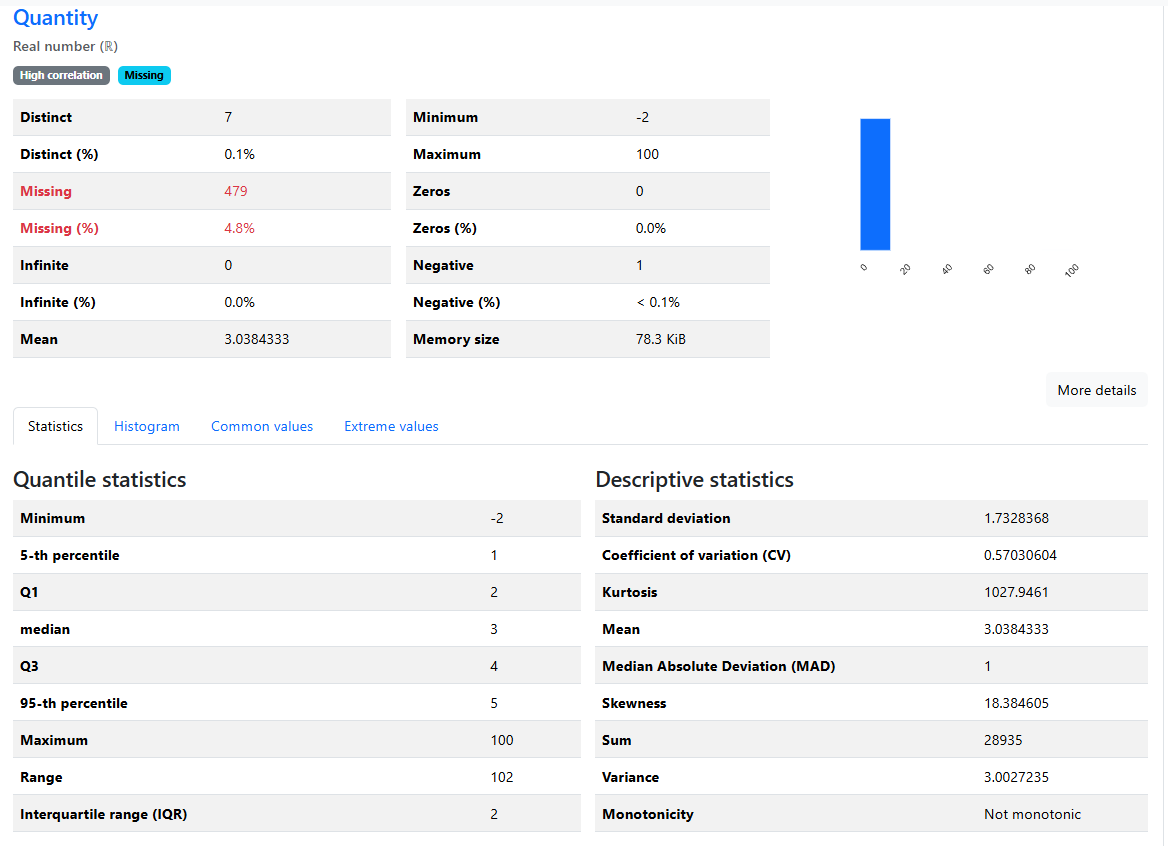
\includegraphics[width=0.65\textwidth]{images/py_3.png}
  \caption{Profil kolumny \textit{Quantity}}
\end{figure}

W kolumnie występują anomalnie. Zdarzyła się raz wartość ujemna: -2. Zdarzyła się raz wartość 100, znacznie przekraczająca poza zakres innych (1-5), ale być może dozwolona. Brakuje danych w 4.8\% wierszy. Wartości standardowe, czyli od 1 do 5 włącznie, występują z podobną częstością.

\subsection{Price Per Unit}

\begin{figure}[H]
  \centering
  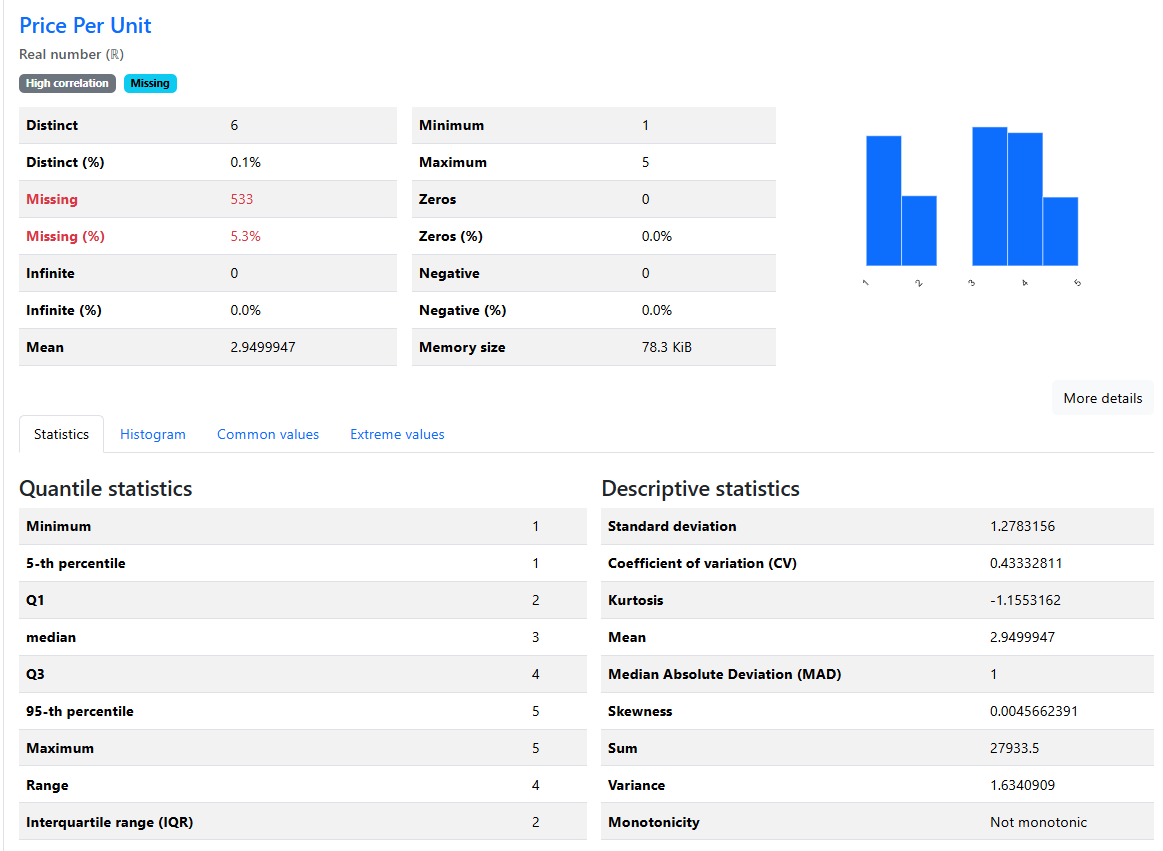
\includegraphics[width=0.65\textwidth]{images/py_4.png}
  \caption{Profil kolumny \textit{Price Per Unit}}
\end{figure}

Kolumna w większości składa się z liczb całkowitych, ale 11.3\% wartości to jedyne z wartością po przecinku. Wszystkie wynoszą dokładnie 1,5. Brakuje wartości dla 5.3\%. Standardowe i jedyne poza brakującymi wartości to liczby całkowite od 1-5 oraz 1,5. Najczęściej występuje wartość 3. Wystepowanie wartości 1,5 jest raczej jednak jak najbardziej dozwolone.

\subsection{Total Spent}

\begin{figure}[H]
  \centering
  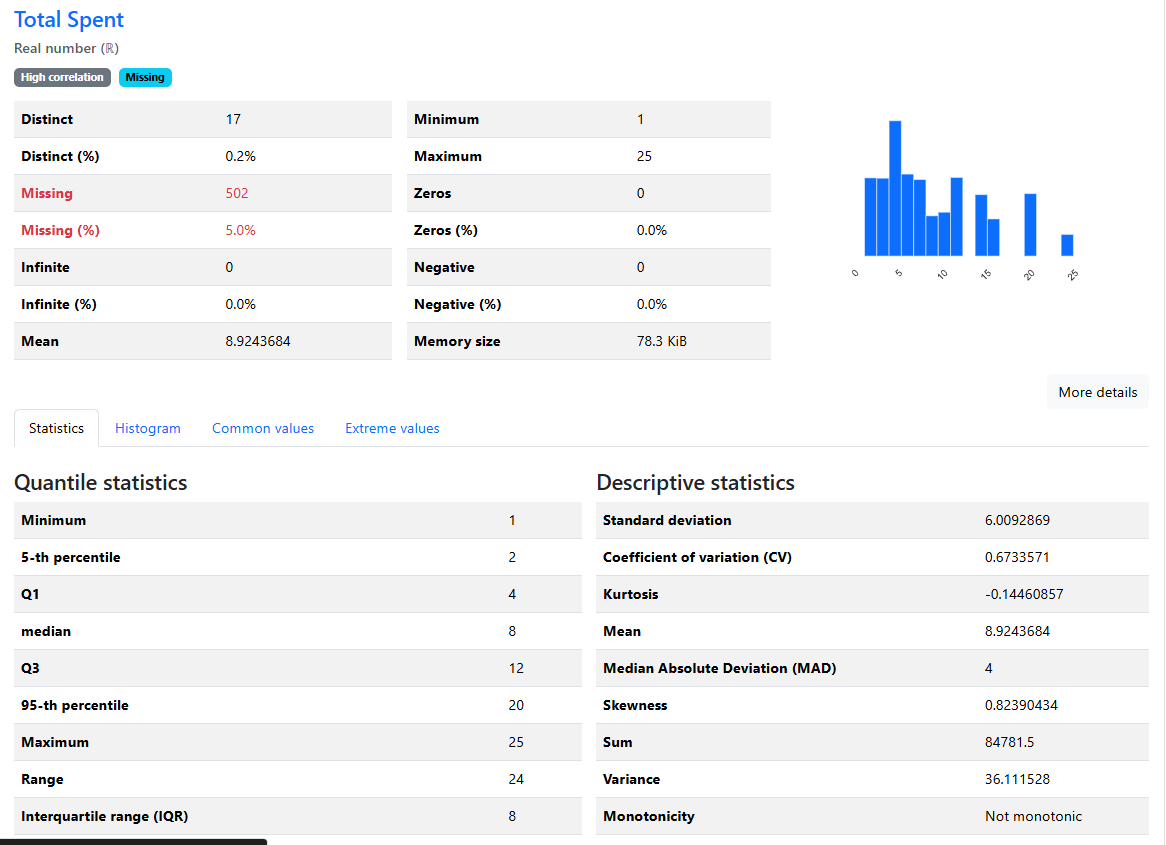
\includegraphics[width=0.65\textwidth]{images/py_5.png}
  \caption{Profil kolumny \textit{Total Spent}}
\end{figure}

Brakuje 5.02\% wartości. Przedział to liczby od 1 do 25 (ale tylko 17 z nich jest w danych). Większość wartości to liczby całkowite, ale występują też wielokrotności 1,5, sugerując, że cena 1,5 w Price Per Unit nie jest żadną anomalią. Najczęściej występuje wartość 6. Większość wartości jest bliżej początku rozkładu niż końca. Po dodatkowej analizie okazało się, że w 1 przypadku Total Spent został źle policzony.

\subsection{Payment Method}

\begin{figure}[H]
  \centering
  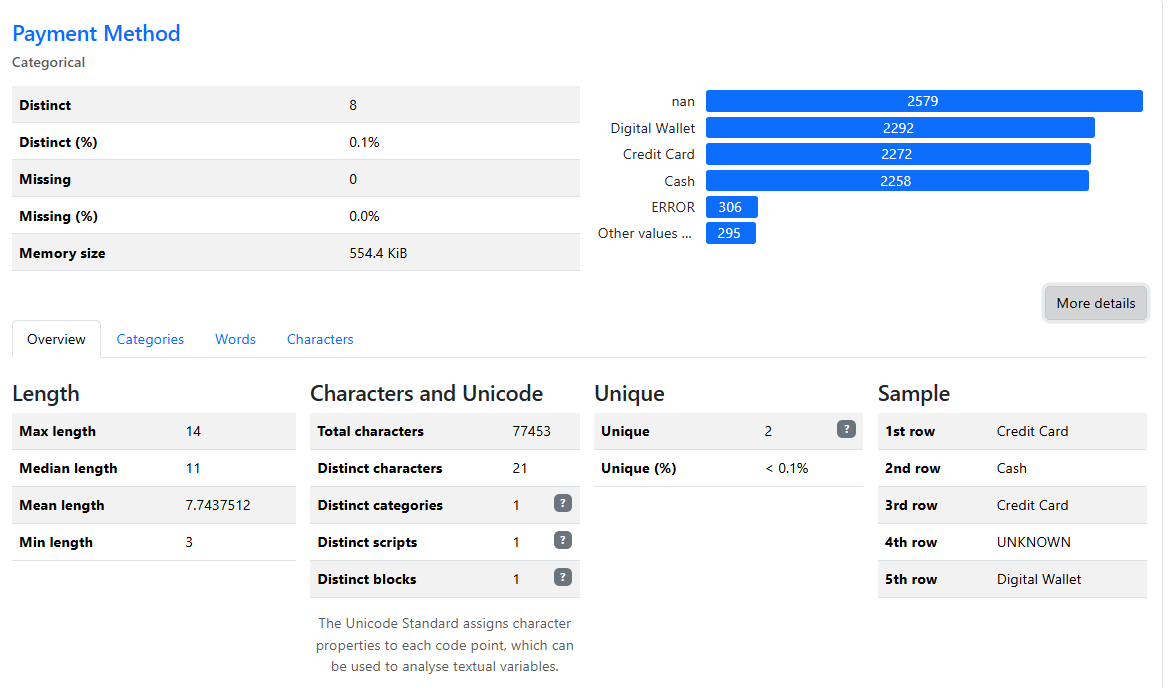
\includegraphics[width=0.65\textwidth]{images/py_6.png}
  \caption{Profil kolumny \textit{Payment Method}}
\end{figure}

Niepoprawne to 31,78\% całości - połaczenie \textit{nan}, \textit{ERROR} i \textit{UNKNOWN}. Oczywiście przy odczytywaniu karty mogą zdarzać się błędy, ale wtedy transakcje raczej powinny być odrzucane i nie znajdować się w bazie danych. Dodatkowo 2 razy wystąpiły literówki - Digital Walle i CreditCard zamiast Digital Wallet i Credit Card (występujących znacznie częściej). Poprawne kategorie to Digital Wallet, Credit Card	i Cash.

\subsection{Location}

\begin{figure}[H]
  \centering
  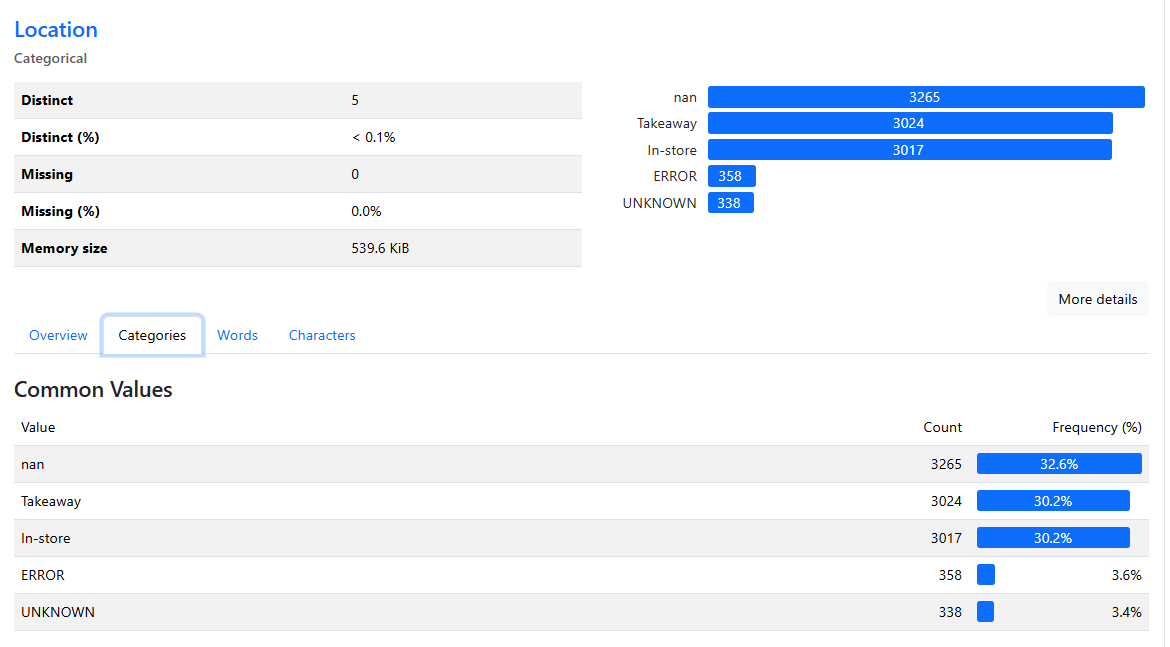
\includegraphics[width=0.65\textwidth]{images/py_7.png}
  \caption{Profil kolumny \textit{Location}}
\end{figure}

Podobnie jak poprzednio, wielu danych brakuje. Nan, ERROR i UNKNOWN występują z częstością 39,61\%. Poza tym, 2 poprawne kategorie to Takeaway lub In-store.

\subsection{Transaction Date}

\begin{figure}[H]
  \centering
  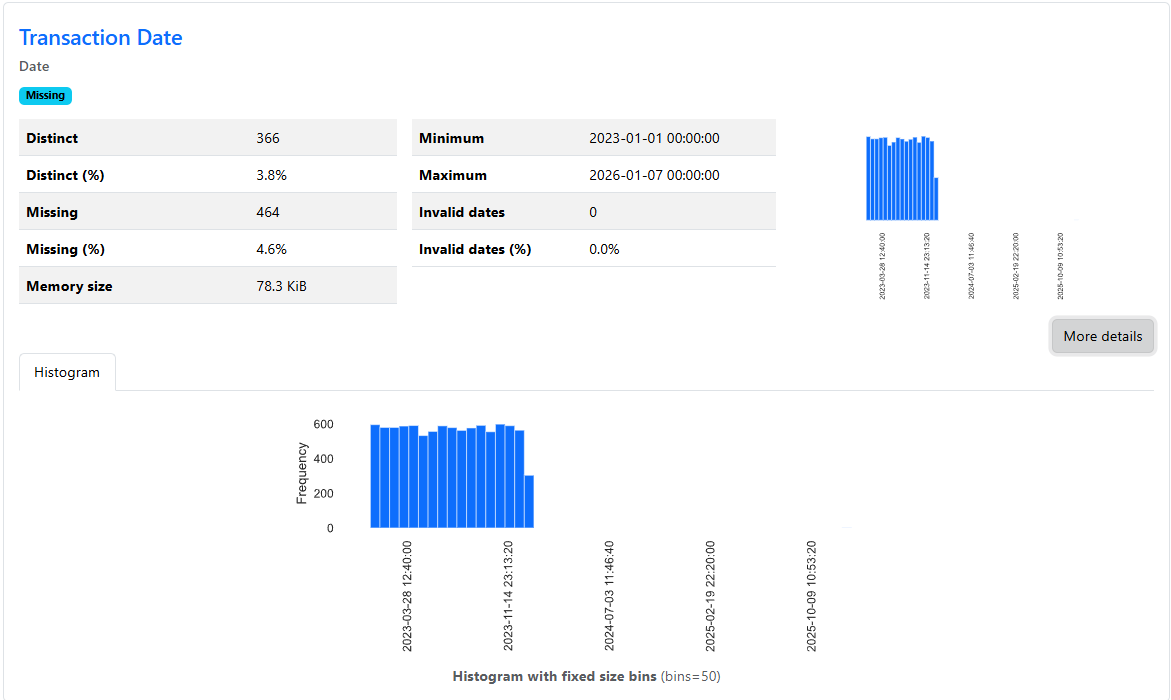
\includegraphics[width=0.65\textwidth]{images/py_8.png}
  \caption{Profil kolumny \textit{Transaction Date}}
\end{figure}

Przez jedną literówkę w danych zakres wydaje się być od 2023-01-01 do 2026-01-07. Rzeczywiście jednak dane są od 2023-01-01 do 2023-12-31, a wystąpiła literówka w 2026 i rok powinien zostać zmieniony na 2023. Poza tym rozkład jest dość równomierny, jedynie w grudniu jest wyraźny spadek. Brakuje 4,6\% wartości.

\subsection{Przykład interakcji}

\begin{figure}[H]
  \centering
  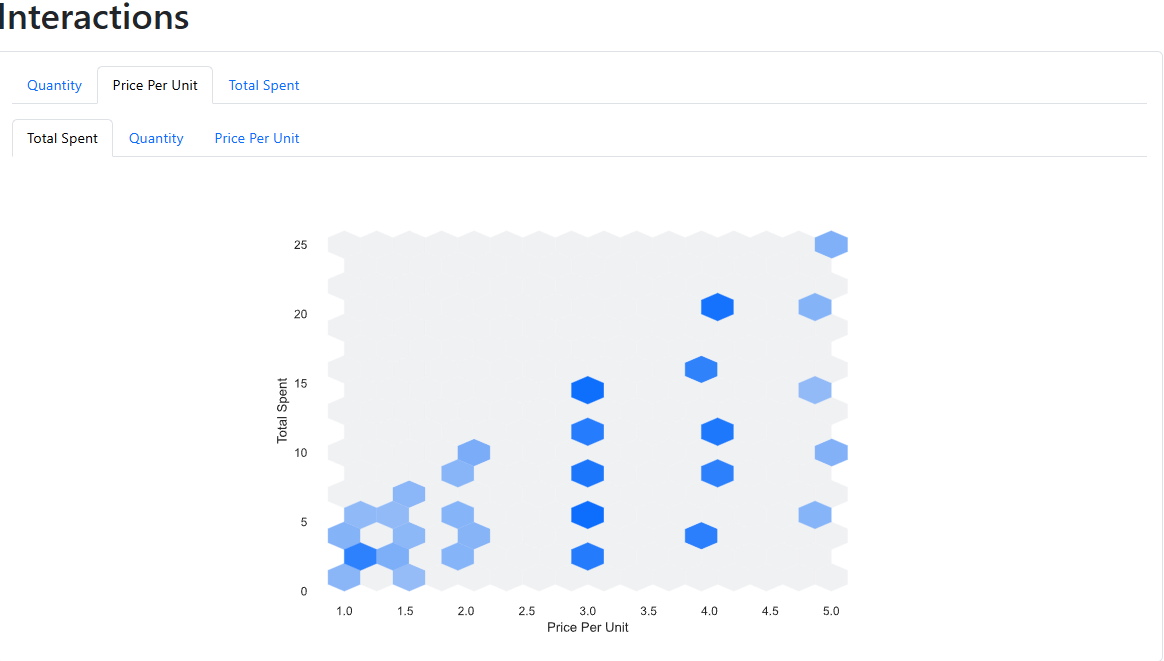
\includegraphics[width=0.65\textwidth]{images/py_interactions_example.png}
  \caption{Przykład interakcji między Price Per Unit a Total Spent}
\end{figure}

Jak widać, występuje pozytywna korelacja miedzy Price Per Unit a Total Spent.

\section{Wnioski}

\subsection{Wnioski z zadania 1}

Klienci bardzo różnią się miedzy sobą. Niektórzy wydają tylko w jednym roku niskie sumy, inni wydają na przestrzeni lat duże pieniądze. Ostatecznie sprowadza się to do wysokich przychodów firmy, rosnących między 2011-2013. Jest szansa na utrzymanie tego trendu w 2014 roku.

Wiele produktów nigdy nie miało rabatu. Najwięcej rabatów udzielono w 2013 roku, ale ta wartość i tak jest niska, biorąc pod uwagę przychody firmy.
Zdecydowanie najwięcej rabatów udzielono na rowery - reszta kategorii nie osiągnęła sumarycznie nawet 10\% sumy rabatów dla rowerów.

\subsection{Wnioski z zadania 2}

Podobnie jak wcześniej widać trendy firmy - przychodów rosnących między 2011-2013. W 2014 roku najbardziej spadła sprzedaż komponentów, a najmniej akcesoriów.

Tak jak w poprzednim raporcie zauważono, nie każdy sprzedawca obsługuje tyle samo transakcji co inny w danym roku. Na przykład, Syed Abbas w 2013 roku obsłużył 12 transakcji, a w 2014 tylko 4. Dla porównania Michael Blythe obsłużył w 2011 65 transakcji, w 2012 - 148, 2013 - 175 a w 2014 - 62.

W tym przypadku DENSE\_RANK wygląda lepiej niż RANK. Oba ostatecznie funkcjonują tak samo, ale wielu klientów ma tą samą liczbę transakcji (na przykład 2). Powoduje to okazjonalne duże skoki w miejscach rankingowych. W DENSE\_RANK to zjawisko nie występuje. Zdecydowana większość klientów wykonała mało transakcji, ale 746 (na 19119) klientów wykonało ich co najmniej 10. 214 klientów wykonało co najmniej 100 transakcji, a rekordzistą jest Reuben D'sa z 530 transakcjami.

Do zadania 2.4 należało oczywiście użyć funkcji NTILE. Warto byłoby zobaczyć porównaniu między rankingiem opartym na średniej liczbie sprzedanych sztuk a sumą liczby sprzedanych sztuk/sumą przychodów. Ranking w aktualnej postaci dotyczy tego, ile w tej samej transakcji zakupiono średnio dany produkt. Nie oznacza to, że ten produkt jest faktycznie najbardziej opłacalny dla sklepu.

\subsection{Wnioski z zadania 3}

Jakość danych jest niska i wynika to prawdopodobnie z braku odpowiedniej walidacji w systemie zbierającym dane. Raczej niepoprawne jest przechowywanie w bazie danych transakcji, gdzie wystąpił błąd przy odczycie metody płatności. Możliwe, że dane nie były wpisywane automatycznie, tylko wymagały za każdym razem manualnego wpisu. Występują poważne literówki i błędy, takie jak literówki w kategorii karty, ujemna wartość Quantity czy rok 2026 w Transaction Date.

Największym problemem jest jednak liczba danych, jakiej brakuje - w zależności od kolumny waha się do nawet 40\%. W tylko jednej kolumnie jakość danych jest prawie idealna - Transaction ID ma tylko 3 duplikaty i wszędzie ma wartości. Wykluczając Transaction ID, przedział brakujących wartości wynosi od 3,4\% do 39,61\%.

Najwięcej problemów mają kolumny Location i Payment Method. W Location brakuje 39,61\% danych, a w Payment Method, wliczając ERROR i UNKNOWN 31,78\%. Poza tym, w Payment Method wystąpiła 2 razy literówka.

Te problemy mocno utrudniłyby przeniesienie podanych danych do porządnej bazy danych z zapisem wszystkich wierszy. Dane te jednak można jak najbardziej przeanalizować, a nawet naprawić oczywiste błędy. Literówki w kategoriach karty można łatwo poprawić, usunąć wiersz z ujemną Quantity i poprawić rok 2026 na 2023. Można nawet próbować domyślić się niektórych brakujących wartości - jeśli brakuje tylko 1 wierzchołka w trójkącie Quantity, Price Per Unit i Total Spent, da się go wywnioskować. Bez dodatkowej wiedzy nie będzie można jednak przywrócić innych brakujących danych.

Nowoczesne narzędzia do analizy danych potrafią bardzo mocno i szybko wspomóc proces analityka i inżyniera danych.

\printbibliography

\end{document}